\documentclass[english,engineering]{wizthesis}

\usepackage[utf8]{inputenc}
\usepackage{float} % H float positioning
\usepackage{xcolor}
\usepackage{enumitem} % enumerate
\usepackage{amsmath, bm}
\usepackage{mathtools}
\usepackage[ruled,vlined]{algorithm2e}
\usepackage{wrapfig}
\usepackage{tikz}
\usepackage{tikz-uml}
\usepackage{booktabs}
\usepackage{xltabular}
\usepackage{array} % \raggedright, \arraybackslash

\AtBeginEnvironment{xltabular}{\setlist[enumerate, 1]{wide, leftmargin=*, itemsep=0pt, before=\vspace{-\dimexpr\baselineskip +2 \partopsep}, after=\vspace{-\baselineskip}}}

% Set up the thesis
\author{Karol Belina}
\title{Formal grammar\par production rule parsing tool}
\supervisor{dr inż. Zdzisław Spławski}
\fieldofstudy{Computer Science}
\keywords{Parser combinators, context-free grammars, Extended Backus-Naur Form}
\summary{The thesis documents the process of designing and implementing a tool
for parsing the production rules of context-free grammars in a textual form. It
discusses the choice of Extended Backus-Naur Form notation over the alternatives
and provides a mathematical model for parsing such a notation. The implemented
parser can turn a high-level specification of a grammar into a parser itself,
which in turn is capable of constructing a parse tree from arbitrary input
provided to the program with the use of parser combinators.}

% Set up the bibliography style
\bibliographystyle{acm}
% Set up the column types
\newcolumntype{L}[1]{%
  >{\raggedright\let\newline\\\arraybackslash\hspace{0pt}}p{#1}%
}

\newcommand{\todo}[1]{%
  \textcolor{red}{[\textbf{TODO}\ifx&#1&{}\else{ }\fi\emph{#1}]}%
}

\begin{document}

\frontmatter % Disable page and chapter numbering for this section

\maketitle

% '\chapter*' removes both abstracts from the table of contents
\chapter*{Abstract}

The thesis presents the design and implementation of a context-free grammar
parsing tool with real-time explanations and error detection. It discusses the
choice of Extended Backus-Naur Form notation over the alternatives and provides
a mathematical model for parsing such a notation. For this purpose, the official
specification of the EBNF from the ISO/IEC 14977 standard has been examined and
transformed into an unambiguous form. A definition of a grammar is proposed to
act as a result of the syntactic analysis phase formed with a technique called
\emph{parser combination}. A method of testing an arbitrary input against the
language generated by the constructed grammar is described. The thesis shows the
process of creating a simple command line REPL program to act as a basic tool
for interfacing with the grammar parser and checker, but in order to efficiently
use the library, a web-based application is designed on top of that to serve as
a more visual, user-friendly and easily accessible tool. It describes the
deployment of the application on a static site hosting service, as well as a
cross-platform desktop application. The designed and implemented system gives
the opportunity to extend it with other grammar specifications.

{\let\clearpage\relax % Keep the polish abstract on the same page
\chapter*{Streszczenie}

Praca przedstawia proces projektowania i~implementacji narzędzia służącego~do
analizy~syntaktycznej gramatyk~bezkontekstowych z~naciskiem na~obsługę błędów
i~wyjaśnień w czasie rzeczywistym. Omawia wybór rozszerzonej~notacji
Backusa-Naura i~przestawia matematyczny model do~analizy takiej notacji. W~tym
celu przeprowadzono analizę i~przekształcenie w jednoznaczną formę oficjalnej
jej specyfikacji zdefiniowanej w standardzie ISO/IEC~14977. Zaproponowana
zostaje definicja gramatyki tej notacji, która jest tworzona w wyniku analizy
syntaktycznej za pomocą techniki zwanej \emph{kombinacją~parserów}. Opisana
zostaje metoda sprawdzania dowolnego ciągu znaków pod kątem języka generowanego
przez analizowaną gramatykę. Praca przedstawia stworzenie prostego programu
działającego z~poziomu wiersza poleceń, który jest podstawowym narzędziem do
analizy gramatyk, jednak by móc efektywnie korzystać ze~stworzonej biblioteki,
zaprojektowana zostaje aplikacja webowa, która służy za bardziej wizualne,
przyjazne i łatwo dostępne dla użytkownika narzędzie. Praca opisuje wdrażanie
aplikacji na~usługę hostingową dla statycznych stron, a~także jako
wieloplatformowej aplikacji. Zaprojektowany i~wdrożony system daje możliwość
rozszerzenia go o~inne specyfikacje gramatyk.}

\tableofcontents

\mainmatter % Re-enable page and chapter numbering

\chapter{Problem analysis}

\section{Description and motivation} \label{sec:description-and-motivation}

Programming language theory has become a well-recognized branch of computer
science that deals with the study of programming languages and their
characteristics. It is an active research field, with findings published in
various journals, as well as general publications in computer science and
engineering. But besides the formal nature of Programming language theory, many
amateur programming language creators try their hand at the challenge of
creating a programming language of their own as a personal project. It is
certainly relevant for a person to write their own language for educational
purposes, and to learn about programming language and compiler design. However,
the language creator must first of all make some fundamental decisions about the
paradigms to be used, as well as the syntax of the language.

The tools for aiding the design and implementation of the syntax of a language
are generally called \emph{compiler-compilers}. These programs create parsers,
interpreters or compilers from some formal description of a programming
language (usually a grammar). The most commonly used types of
compiler-compilers are \emph{parser generators}, which handle only the
syntactic analysis of the language --- they do not handle the semantic analysis,
nor the code generation aspect. The parser generators most generally transform a
grammar of the syntax of a given programming language into a source code of a
parser for that language. The language of the source code for such a parser is
dependent on the parser generator.

Most such tools, however, \todo{offer} too much complexity and generally have a steep
learning curve for people inexperienced with the topic. Limited availability
makes them less fitted for prototyping a syntax of a language --- they often
require a complex setup for simple tasks, which is not welcoming for new users
\todo{and may lead to...?}. The lack of visualization capabilities shipped with
these tools makes them less desirable for teachers in the theory of formal
languages, who often require such features for educative purposes in order to
present the formulations of context-free grammars in a more visual format.

\section{Goal of the thesis}

The main goal of this thesis is to design and implement a specialized tool, that
serves teachers, programmers and other kinds of enthusiasts of the theory of
formal languages in the field of discrete mathematics and computer science, in
order to formulate and visualize context-free grammars in the form of the
Extended Backus-Naur Form. In order to \todo{}, the tool must provide a
graphical user interface. Additionally, to ensure the hightest degree of
accessibility, the tool must be available in the form of an easily accessible
web-based application that is accessed through a web page and can run in a
browser without the need of installation on the user's device. The thesis itself
will document the entire process of creating such a project.

\todo{jak projekt pomoże w powyższych problemach?}

In order to achieve the general goal, several sub-goals have been
distinguished, all of which contribute to the main objective as a whole
\begin{itemize}
  \item analysis of existing solutions and applications,
  \item presentation of the theoretical preliminaries of the project,
  \item definition of the outline of the project, including a description of
  the functional and non-functional requirements, the use case diagram, use case
  scenarios, the class diagram, and the user interface prototype,
  \item description of technologies used in the implementation,
  \item implementation of the project,
  \item description of the testing and deployment environments.
\end{itemize}

\section{Scope of the project}

The thesis will propose a definition of a grammar in the form of an abstract
syntax tree of the Extended Backus-Naur Form. It will describe the process of
implementing the business logic of the application in the Rust programming
language compiled to WebAssembly. The compiled code is then ran inside the
web-based application made with the Svelte framework, which incorporates the
markup, CSS styles, and JavaScript scripts in the superset of the HyperText
Markup Language (HTML).

The implementation phase will include the process of tokenization --- the act of
dividing the grammar in a textual form into a sequence of tokens --- while
taking into account proper interpretation of Unicode graphemes. The
whitespace-agnostic tokens will be then combined together to form a
previously-defined abstract syntax tree with a technique called \emph{parser
combination}. Several smaller helper parsers will be defined, all of which then
will be combined into more sophisticated parsers capable of parsing entire
terms, productions, and grammars. The implementation phase will also include the
definition of an algorithm for handling left recursion in the resulting grammar,
as well as a dependency graph reduction algorithm for determining the starting
rule of a grammar. Up to this stage, any errors encountered in the textual form
of a grammar are going to be reported to the user in a friendly format with
exact locations of the errors in the input.

\todo{\begin{itemize}[noitemsep,nolistsep]
  \item service workers
  \item wizualizacje, edytor tekstowy i kolorowanie składni
  \item wyjaśnienia zwracane przez checker?
  \item wyrażenia regularne w specjalnych sekwencjach?
\end{itemize}}

The web application will be deployed on the GitHub Pages hosting service for
static sites, as well as a standalone desktop application with the use of the
Electron framework.

\section{Glossary}

\begin{description}[leftmargin=!,labelwidth=2cm]
  \item[AST] Abstract syntax tree --- \todo{},
  \item[EBNF] Extended Backus-Naur Form --- \todo{},
  \item[parser] \todo{},
  \item[REPL] Read-Eval-Print loop --- \todo{}.
  \item \todo{}
\end{description}

\chapter{Theoretical preliminaries}

\section{Formal grammars}

\subsection{Introduction to formal grammars}

\emph{Formal grammar} of a language defines the construction of strings of
symbols from the language's \emph{alphabet} according to the language's
\emph{syntax}. It is a set of so-called \emph{production~rules} for
rewriting certain strings of symbols with other strings of symbols --- it can
therefore generate any string belonging to that language by repeatedly applying
these rules to a given starting symbol~\cite{meduna-2014}. Furthermore, a
grammar can also be applied in reverse: it can be determined if a string of
symbols belongs to a given language by breaking it down into its constituents
and analyzing them in the process known as \emph{parsing}.

For now, let's consider a simple example of a formal grammar. It consists of two
sets of symbols: (1) set $N = \{\,S, B\,\}$, whose symbols are
\emph{non-terminal} and must be rewritten into other, possibly non-terminal,
symbols, and (2) set $\Sigma = \{\,a, b, c\,\}$, whose symbols are
\emph{terminal} and cannot be rewritten further. Let $S$ be the start symbol
and set $P$ be the set of the following production rules:
\begin{enumerate}[noitemsep]
  \item $S \rightarrow aBSc$
  \item $S \rightarrow abc$
  \item $Ba \rightarrow aB$
  \item $Bb \rightarrow bb$
\end{enumerate}
To generate a string in this language, one must apply these rules (starting with
the start symbol) until a string consisting only of terminal symbols is
produced. A production rule is applied to a string by replacing an occurrence
of the production rule's left-hand side in the string by that production rule's
right-hand side. The simplest example of generating such a string would be
\begin{equation*}
  S \xRightarrow[2]{} \underline{abc}
\end{equation*}
where $P \xRightarrow[i]{} Q$ means that string $P$ generates the string $Q$
according to the production rule $i$, and the generated part of the string
is underlined.

By choosing a different sequence of production rules we can generate a different
string in that language
\begin{equation*}
\begin{split}
  S & \xRightarrow[1]{} \underline{aBSc} \\
    & \xRightarrow[2]{} aB\underline{abc}c \\
    & \xRightarrow[3]{} a\underline{aB}bcc \\
    & \xRightarrow[4]{} aa\underline{bb}cc
\end{split}
\end{equation*}

After examining further examples of strings generated by these production rules
we may come into a conclusion that this grammar generates the language
$\{\,a^nb^nc^n \mid n \ge 1\,\}$, where $x^n$ is a string of $n$ consecutive $x$'s.
It means that the language is the set of strings consisting of one or more
$a$'s, followed by the exact same number of $b$'s, then followed by the exact
same number of $c$'s.

Such a system provides us with a notation for describing a given
language formally. Such a language is a usually infinite set of finite-length
sequences of terminal symbols from that language.

\subsection{The Chomsky Hierarchy}

\begin{wrapfigure}{R}{0.45\textwidth}
  \centering
  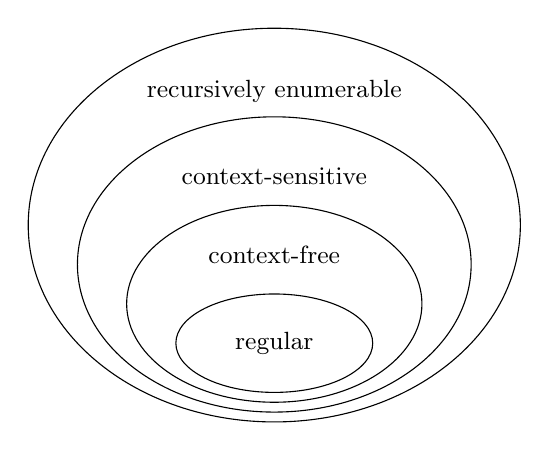
\begin{tikzpicture}[scale=2.5]
    \draw[color=black](0,0) ellipse (1.25 and 1)
      node at (0, 0.68) {\small recursively enumerable};
    \draw[color=black](0,-0.2) ellipse (1 and 0.75)
      node at (0, 0.25) {\small context-sensitive};
    \draw[color=black](0,-0.4) ellipse (0.75 and 0.5)
      node at (0, -0.15) {\small context-free};
    \draw[color=black](0,-0.6) ellipse (0.5 and 0.25)
      node {\small regular};
  \end{tikzpicture}
  \caption{The~Chomsky~Hierarchy visualized}
  \label{fig:chomsky-hierarchy}
\end{wrapfigure}

In~\cite{chomsky-1956} Chomsky divides formal grammars into four classes and
classifies them in the now called \emph{Chomsky~Hierarchy}. Each class is a
subset of another, distinguished by the complexity.

Type-3 grammars generate the so-called \emph{regular~languages}. As described
in~\cite{aho-1990}, regular languages can be matched by
\emph{regular~expressions} and decided by a \emph{finite~state~automaton}.
They are the most restricting kinds of grammars, with its production rules
consisting of a single non-terminal on the left-hand side and a single terminal,
possibly followed by a single non-terminal on the right-hand side. Because of
their simplicity, regular languages are used for lexical analysis of programming
languages~\cite{johnson-1968}.

Type-2 grammars produce \emph{context-free~languages} and can be represented
as a \emph{pushdown~automaton} which is an automaton that can maintain its
state with the use of a stack. \todo{jak w stosie wygląda pamięć}

\subsection{Parsing Expression Grammars}

\todo{\url{https://en.wikipedia.org/wiki/Parsing_expression_grammar}}

\todo{\cite{ford-2004}}

\section{Why EBNF?}

\todo{}

\section{Modifying the specification}

\todo{analiza i zmodyfikowanie oficjalnej specyfikacji EBNF}

See appendix \ref{ch:modified-spec}.

\section{Methods of syntactic analysis} \label{sec:parsing}

\subsection{Bottom-up parsing}

\todo{}

\subsection{Top-down parsing and parser combination}

\todo{opisanie parser combinatorów (w Haskellu?) \cite{swierstra-2009}
\cite{leijen-2001} \cite{fokker-1995}}

\begin{minted}{haskell}
type Parser a = String -> Maybe (a, String)
\end{minted}

% \begin{minted}{haskell}
% parse digit "123"
% -- Just ('1', "23")
% \end{minted}

% \begin{minted}{haskell}
% parse (char 'a') "bcd"
% -- Nothing
% \end{minted}

% \begin{minted}{haskell}
% parse (multiple (digit <|> letter)) "abc123"
% -- Just ("abc123", "")
% \end{minted}

\chapter{Analysis of similar solutions}

\section*{Coco/R}

\todo{\cite{coco/r}}

\section*{ANTLR}

\todo{\cite{antlr}}

\section*{Bison}

\todo{\cite{bison}}

\section*{PLY}

\todo{\cite{ply}}

\section*{Regex101}

\todo{\cite{regex101}}

\chapter{Design of the project}

\section{Requirements}

\subsection{Functional requirements}

\begin{xltabular}{\textwidth}{@{}lL{3cm}Xl@{}}
  \caption{The functional requirements of the project, their features, and
  priorities}
  \label{tab:functional-requirements}\\
  \toprule
  Id & Requirement & Features & Priority \\* \midrule
  \endfirsthead
  %
  \endhead
  %
  \endfoot
  %
  \endlastfoot
  %
  \emph{FR1} & Specifying the grammar & The user can specify the grammar of a
  given language in the EBNF notation by providing it in a textual form in
  a designated editor window. & high \\
  \addlinespace[0.5em] \emph{FR2} & Error reporting & The editor provides
  feedback about any syntactic or semantic errors encountered during the
  parsing by highlighting the exact location of the error in the provided
  grammar. The user can then hover the mouse pointer over the highlighted area
  to read the error message. & high \\
  \addlinespace[0.5em] \emph{FR3} & Specifying the input string & The user can
  specify the input string in a designated editor window to check if it
  belongs to the language generated by the previously-defined grammar. & high
  \\
  \addlinespace[0.5em] \emph{FR4} & Visualizing the parse tree & The
  application visualizes the parse tree resulting from parsing the specified
  input string with the parser generated by the grammar defined by the user. &
  high \\
  \addlinespace[0.5em] \emph{FR5} & Syntax highlighting & The editor highlights
  parts of the specified grammar with a different syntactic meaning in a
  different manner with the use of multi-colored fonts. & medium \\
  \addlinespace[0.5em] \emph{FR6} & Autocompletion of non-terminals & The
  editor predicts the identifier of a non-terminal a user is typing by
  providing a list of possible non-terminals, which then can be chosen by the
  user. & low \\
  \addlinespace[0.5em] \emph{FR7} & Production rule folding & The editor
  provides the ability to hide and reveal a production rule of the grammar
  inside the editor window. & low \\
  \addlinespace[0.5em] \emph{FR8} & Search and replace interface & The user can
  search for any occurrences of a phrase in the editor window and possibly
  replace them with a different phrase. The search and replace functionality
  should also support regular expressions. & low \\* \bottomrule
\end{xltabular}

\newpage

\subsection{Non-functional requirements}

\begin{xltabular}{\textwidth}{@{}Xl@{}}
  \caption{The non-functional requirements of the project and their priorities}
  \label{tab:non-functional-requirements}\\
  \toprule
  Requirement & Priority \\* \midrule
  \endfirsthead
  %
  \endhead
  %
  \endfoot
  %
  \endlastfoot
  %
  The web application should be available 24 hours a day, 7 days a week. &
  medium \\
  \addlinespace[0.5em] Page loading time should be less than 1 second with
  internet download speed of 80\,Mbps. Parsing and checking times should both
  be less than 50 milliseconds. & high \\
  \addlinespace[0.5em] The application must work and display correctly in
  \begin{itemize}[noitemsep,nolistsep]
    \item Chrome version 86 or later,
    \item Safari version 14 or later,
    \item Edge version 86 or later,
    \item Firefox version 82 or later,
    \item Opera version 71 or later, \end{itemize} as well as in the Electron
  framework version v10.1.5. & high \\
  \addlinespace[0.5em] Usability \todo{} % This focuses on the appearance of
  % the user interface and how people interact with it. What colour are the
  % screens? How big are the buttons?
  & medium \\
  \addlinespace[0.5em] The source code of the product should be open source
  and freely available for possible modification and redistribution. & high \\
  \addlinespace[0.5em] The project should include the documentation necessary
  for extension and maintenance of the system. & high \\
  \addlinespace[0.5em] The system should provide high degree of integrability
  with future components which extend the functionalities of the system. & high
  \\* \bottomrule
\end{xltabular}

\section{User stories}

\begin{xltabular}{\textwidth}{@{}lX@{}}
  \caption{The user stories}
  \label{tab:user-stories}\\
  \toprule
  Id & User story \\* \midrule
  \endfirsthead
  %
  \endhead
  %
  \endfoot
  %
  \endlastfoot
  %
  \emph{US1} & As the user, I want to be able to paste the contents of my
  clipboard into the editor window in the application. \\
  \addlinespace[0.5em] \emph{US2} & As the user, I want to be able to type in
  the editor window with my keyboard. \\
  \addlinespace[0.5em] \emph{US3} & As the user, I want to be able to appreciate
  the multi-colored appearance of the text that represents the syntax that I
  provided. \\
  \addlinespace[0.5em] \emph{US4} & As the user, I want to be able to select a
  portion of the text in the editor window and copy it to the clipboard using a
  keyboard shortcut. \\
  \addlinespace[0.5em] \emph{US5} & As the user, I want to be able to hold the
  \emph{Alt} key on my keyboard to create multiple cursors in the editor window.
  \\
  \addlinespace[0.5em] \emph{US6} & As the user, I want to have the ability to
  autocomplete the non-terminal I am typing that has already been declared
  elsewhere in the code. \\
  \addlinespace[0.5em] \emph{US7} & As the user, I want to be able to hide any
  existing production rules that might appear too long, to increase the degree
  of clarity and readability of the grammar I'm working on. \\
  \addlinespace[0.5em] \emph{US8} & As the user, I want to be able to show any
  previously hidden production rules of the grammar. \\
  \addlinespace[0.5em] \emph{US9} & As the user, I want to have the ability to
  press a certain key combination on my keyboard that would allow be to type a
  specific phrase in the popup window, which would then find all the occurrences
  of that phrase in the editor window. \\
  \addlinespace[0.5em] \emph{US10} & As the user, I want to be able to provide a
  regular expression for the \emph{find} functionality that would allow me to
  find all occurrences of phrases that pattern match that specific regular
  expression. \\
  \addlinespace[0.5em] \emph{US11} & As the user, I want to be able to replace
  some of the occurrences of phrases found with the \emph{find} functionality
  with another phrase provided in a popup window. \\
  \addlinespace[0.5em] \emph{US12} & As the user, I want to be able to specify
  the initial production rule in the process of checking the input string
  against the grammar I provided. \\
  \addlinespace[0.5em] \emph{US13} & As the user, I want to be able to see
  errors in the syntax of the provided grammar in the form of underlined text in
  the location of where the errors actually occur. \\
  \addlinespace[0.5em] \emph{US14} & As the user, I want to have the ability to
  hover the mouse pointer over the underlined text to read the error message at
  that location. Alternatively, I want to be able to hover over the error
  indicator, which appears next to the line number. \\
  \addlinespace[0.5em] \emph{US15} & As the user, I want to be able to see the
  parse tree of the recognized input string that I provided. \\
  \addlinespace[0.5em] \emph{US16} & As the user, I want to have the ability to
  collapse any nodes in the visualized parse tree that might appear too long.
  \\* \bottomrule
\end{xltabular}

\section{Use case specification}

\subsection{Use cases}

\begin{figure}[H]
  \centering
  \resizebox{0.9\textwidth}{!}{%
    \begin{tikzpicture}
      \tikzumlset{fill usecase=white}
      \begin{umlsystem}{System}
        \umlusecase[x=2,y=3,width=2cm]{Specifying the grammar}
        \umlusecase[x=-2,y=3,width=2cm]{Specifying the input string}
        \umlusecase[x=-2,y=0,width=2cm]{Interacting with the visualization}
        \umlusecase[x=2,y=0,width=2.5cm]{Changing the initial rule}
      \end{umlsystem}

      \umlactor[x=-6,y=0]{User}

      \umlassoc{User}{usecase-1}
      \umlassoc{User}{usecase-2}
      \umlassoc{User}{usecase-3}
      \umlextend[name=incl]{usecase-1}{usecase-4}

      \umlnote[x=8,fill=white,width=4.5cm]{incl-1}{\emph{condition:} \{user specified at least one production rule\}\\
      \emph{extension point:} Initial rule specification}
    \end{tikzpicture}
  }
  \caption{The use case diagram}
  \label{fig:use-case-diagram}
\end{figure}

\begin{xltabular}{\textwidth}{@{}lL{3cm}Xl@{}}
  \caption{Descriptions of the use cases}
  \label{tab:use-cases}\\
  \toprule
  Id & Name & Description \\* \midrule
  \endfirsthead
  %
  \endhead
  %
  \endfoot
  %
  \endlastfoot
  %
  \emph{UC1} & Specifying the grammar & Allows the user to specify the grammar
  of a given language in the EBNF notation by providing it in a textual form in
  a designated editor window. \\
  \addlinespace[0.5em] \emph{UC2} & Specifying the input string & Allows the
  user to specify the input string in a designated editor window to check if it
  belongs to the language generated by the previously-defined grammar. \\
  \addlinespace[0.5em] \emph{UC3} & Interacting with the visualization & Allows
  the user to observe the visualized parse tree of the provided input string and
  interact with it by expanding and collapsing the tree nodes. \\
  \addlinespace[0.5em] \emph{UC4} & Changing the initial rule & Allows the user
  to specify the initial production rule used in the process of checking the
  provided input string against the defined grammar. \\* \bottomrule
\end{xltabular}

\subsection{Requirements traceability graph}

\begin{figure}[H]
  \centering
  \pgfdeclarelayer{bg}
  \pgfsetlayers{bg,main}
  \resizebox{\textwidth}{!}{%
    \begin{tikzpicture}[xscale=1.2,yscale=3]
      \tikzstyle{every node}=[draw,circle,minimum size=1cm,inner sep=0pt,fill=white]

      \node at (-1.5,-1) (uc1) {\emph{UC1}};
      \node at (-0.5,-1) (uc2) {\emph{UC2}};
      \node at (0.5,-1)  (uc3) {\emph{UC3}};
      \node at (1.5,-1)  (uc4) {\emph{UC3}};

      \node at (-7.5,0) (us1)  {\emph{US1}};
      \node at (-6.5,0) (us2)  {\emph{US2}};
      \node at (-5.5,0) (us3)  {\emph{US3}};
      \node at (-4.5,0) (us4)  {\emph{US4}};
      \node at (-3.5,0) (us5)  {\emph{US5}};
      \node at (-2.5,0) (us6)  {\emph{US6}};
      \node at (-1.5,0) (us7)  {\emph{US7}};
      \node at (-0.5,0) (us8)  {\emph{US8}};
      \node at (0.5,0) (us9)  {\emph{US9}};
      \node at (1.5,0) (us10) {\emph{US10}};
      \node at (2.5,0) (us11) {\emph{US11}};
      \node at (3.5,0) (us12) {\emph{US12}};
      \node at (4.5,0) (us13) {\emph{US13}};
      \node at (5.5,0) (us14) {\emph{US14}};
      \node at (6.5,0) (us15) {\emph{US15}};
      \node at (7.5,0) (us16) {\emph{US15}};

      \node at (-3.5,1) (fr1) {\emph{FR1}};
      \node at (-2.5,1) (fr2) {\emph{FR2}};
      \node at (-1.5,1) (fr3) {\emph{FR3}};
      \node at (-0.5,1) (fr4) {\emph{FR4}};
      \node at (0.5,1)  (fr5) {\emph{FR5}};
      \node at (1.5,1)  (fr6) {\emph{FR6}};
      \node at (2.5,1)  (fr7) {\emph{FR7}};
      \node at (3.5,1)  (fr8) {\emph{FR8}};
      
      \begin{pgfonlayer}{bg}
        \draw (fr1) -- (us1);
        \draw (fr1) -- (us2);
        \draw (fr1) -- (us4);
        \draw (fr1) -- (us5);
        \draw (fr2) -- (us13);
        \draw (fr2) -- (us14);
        \draw (fr3) -- (us1);
        \draw (fr3) -- (us2);
        \draw (fr3) -- (us4);
        \draw (fr3) -- (us5);
        \draw (fr4) -- (us15);
        \draw (fr4) -- (us16);
        \draw (fr5) -- (us3);
        \draw (fr6) -- (us6);
        \draw (fr7) -- (us7);
        \draw (fr7) -- (us8);
        \draw (fr8) -- (us9);
        \draw (fr8) -- (us10);
        \draw (fr8) -- (us11);

        \draw (us1) -- (uc1);
        \draw (us2) -- (uc1);
        \draw (us3) -- (uc1);
        \draw (us4) -- (uc1);
        \draw (us5) -- (uc1);
        \draw (us6) -- (uc1);
        \draw (us7) -- (uc1);
        \draw (us8) -- (uc1);
        \draw (us9) -- (uc1);
        \draw (us10) -- (uc1);
        \draw (us11) -- (uc1);
        \draw (us12) -- (uc1);
        \draw (us13) -- (uc1);
        \draw (us1) -- (uc2);
        \draw (us2) -- (uc2);
        \draw (us3) -- (uc2);
        \draw (us4) -- (uc2);
        \draw (us5) -- (uc2);
        \draw (us6) -- (uc2);
        \draw (us7) -- (uc2);
        \draw (us8) -- (uc2);
        \draw (us9) -- (uc2);
        \draw (us10) -- (uc2);
        \draw (us11) -- (uc2);
        \draw (us13) -- (uc2);
        \draw (us14) -- (uc2);
        \draw (us12) -- (uc3);
        \draw (us15) -- (uc4);
        \draw (us16) -- (uc4);
      \end{pgfonlayer}
    \end{tikzpicture}
  }
  \caption{The requirements traceability graph}
  \label{fig:rtg}
\end{figure}

\subsection{Use case scenarios}

\begin{xltabular}{\textwidth}{@{}L{3cm}X@{}}
  \caption{Use case scenario of \emph{UC1} Specifying the grammar}
  \label{tab:uc1-scenario}\\
  \toprule
  \endfirsthead
  %
  \endhead
  %
  \endfoot
  %
  \endlastfoot
  %
  Identifier & \emph{UC1} \\
  \addlinespace[0.5em] Name & Specifying the grammar \\
  \addlinespace[0.5em] Summary & Allows the user to specify the grammar of a
  given language in the EBNF notation by providing it in a textual form in a
  designated editor window. \\
  \addlinespace[0.5em] Pre-conditions & None. \\
  \addlinespace[0.5em] Post-conditions & The grammar has been correctly defined
  by the user with no syntactic errors. \\
  \addlinespace[0.5em] Main scenario &
  \begin{enumerate}[noitemsep,nolistsep,labelindent=0.5cm,align=right]
    \item [1.] The system shows a grammar editor window to the user.
    \item [2.] The user provides a syntactically and semantically correct
    definition of a grammar.
    \item [3.] The system shows an icon indicating no errors detected in the
    grammar.
    \item [] End of scenario.
  \end{enumerate} \\
  \addlinespace[0.5em] Alternative scenario &
  \begin{enumerate}[noitemsep,nolistsep,labelindent=0.5cm,align=right]
    \item [2a.1.] The user provides an invalid definition of a grammar.
    \item [2a.2.] The system highlights the text in the grammar editor window at
    the error location.
    \item [] Return to step 2.
  \end{enumerate} \\* \bottomrule
\end{xltabular}

\begin{xltabular}{\textwidth}{@{}L{3cm}X@{}}
  \caption{Use case scenario of \emph{UC2} Specifying the input string}
  \label{tab:uc2-scenario}\\
  \toprule
  \endfirsthead
  %
  \endhead
  %
  \endfoot
  %
  \endlastfoot
  %
  Identifier & \emph{UC2} \\
  \addlinespace[0.5em] Name & Specifying the input string \\
  \addlinespace[0.5em] Summary & Allows the user to specify the input string in
  a designated editor window to check if it belongs to the language generated by
  the previously-defined grammar. \\
  \addlinespace[0.5em] Pre-conditions & None. \\
  \addlinespace[0.5em] Post-conditions & The input string has been correctly
  entered by the user. \\
  \addlinespace[0.5em] Main scenario &
  \begin{enumerate}[noitemsep,nolistsep,labelindent=0.5cm,align=right]
    \item [1.] The system shows a input string editor window to the user.
    \item [2.] The user provides a desired input string.
    \item [3.] A valid grammar has been provided by the user in the grammar
    editor window.
    \item [4.] The system shows the result of the checker in the result window.
    \item [] End of scenario.
  \end{enumerate} \\
  \addlinespace[0.5em] Alternative scenario &
  \begin{enumerate}[noitemsep,nolistsep,labelindent=0.5cm,align=right]
    \item [3a.1.] The user did not provide a valid grammar in the grammar editor
    window.
    \item [3a.2.] The system does not show a result of the checker.
    \item [] End of scenario.
  \end{enumerate} \\* \bottomrule
\end{xltabular}

\begin{xltabular}{\textwidth}{@{}L{3cm}X@{}}
  \caption{Use case scenario of \emph{UC3} Interacting with the visualization}
  \label{tab:uc3-scenario}\\
  \toprule
  \endfirsthead
  %
  \endhead
  %
  \endfoot
  %
  \endlastfoot
  %
  Identifier & \emph{UC3} \\
  \addlinespace[0.5em] Name & Interacting with the visualization \\
  \addlinespace[0.5em] Summary & Allows the user to observe the visualized parse
  tree of the provided input string and interact with it by expanding and
  collapsing the tree nodes. \\
  \addlinespace[0.5em] Pre-conditions & The user has provided a valid definition
  of a grammar, as well as an input string, that belongs to the language
  generated by that grammar. \\
  \addlinespace[0.5em] Post-conditions & None. \\
  \addlinespace[0.5em] Main scenario &
  \begin{enumerate}[noitemsep,nolistsep,labelindent=0.5cm,align=right]
    \item [1.] \todo{}
    \item [2.] \todo{}
    \item [3.] \todo{}
    \item [] End of scenario.
  \end{enumerate} \\* \bottomrule
\end{xltabular}

\begin{xltabular}{\textwidth}{@{}L{3cm}X@{}}
  \caption{Use case scenario of \emph{UC2} Specifying the input string}
  \label{tab:uc4-scenario}\\
  \toprule
  \endfirsthead
  %
  \endhead
  %
  \endfoot
  %
  \endlastfoot
  %
  Identifier & \emph{UC4} \\
  \addlinespace[0.5em] Name & Changing the initial rule \\
  \addlinespace[0.5em] Summary & Allows the user to specify the initial
  production rule used in the process of checking the provided input string
  against the defined grammar. \\
  \addlinespace[0.5em] Pre-conditions & The user has provided a valid definition
  of a grammar. \\
  \addlinespace[0.5em] Post-conditions & The initial production rule has been
  successfully changed to the desired one. \\
  \addlinespace[0.5em] Main scenario &
  \begin{enumerate}[noitemsep,nolistsep,labelindent=0.5cm,align=right]
    \item [1.] The system shows a button the current initial production rule
    written on top.
    \item [2.] The user clicks on the button.
    \item [3.] The system shows a dropdown menu with a list of all production
    rules defined in the provided grammar.
    \item [4.] The user clicks on an item of the list corresponding to the
    desired initial production rule.
    \item [5.] The system changes the identifier of the initial production rule
    on the button.
    \item [] End of scenario.
  \end{enumerate} \\* \bottomrule
\end{xltabular}

\subsection{Activity diagrams}

\begin{figure}[H]
  \centering
  \begin{tikzpicture}
    \begin{umlstate}[name=Amain, fill=white]{Etat global de l'objet A}
      \begin{umlstate}[name=Bgraph, fill=white]{graphe B}
        \umlstateinitial[name=Binit]
        \umlbasicstate[y=-4, name=test1, fill=white]{test1}
        \umltrans{Binit}{test1}
        \umltrans[recursive=20|60|2.5cm, recursive direction=right to top, arg={op1}, pos=1.5]{test1}{test1}
        \umltrans[recursive=160|120|2.5cm, recursive direction=left to top, arg={op2}, pos=1.5]{test1}{test1}
        \umltrans[recursive=-160|-120|2.5cm, recursive direction=left to bottom, arg={op3}, pos=1.5]{test1}{test1}
        \umltrans[recursive=-20|-60|2.5cm, recursive direction=right to bottom, arg={op4}, pos=1.5]{test1}{test1}
        \umlbasicstate[y=-8, name=test2, fill=white]{test2}
        \umltrans[recursive=-160|-120|2.5cm, recursive direction=left to bottom, arg={op5}, pos=1.5]{test2}{test2}
        \umltrans{test1}{test2}
        \umlstatefinal[x=3, y=-7.75, name=Bfinal]
        \umltrans{test2}{Bfinal}
      \end{umlstate}
      \umlstateinitial[x=6, y=1, name=Ainit]
      \umlVHtrans[anchor2=40]{Ainit}{Bgraph}
      \umlstatefinal[x=6, y=-3.5, name=Afinal]
      \umlHVtrans[anchor1=30]{Bgraph}{Afinal}
      \umlbasicstate[x=6, y=-6, name=visu, fill=white]{Visualisation}
      \umlHVtrans{Bfinal}{visu}
      \umltrans{visu}{Afinal}
      \umltrans[recursive=-20|-60|2.5cm, recursive direction=right to bottom, arg=a, pos=1.5]{visu}{visu}
    \end{umlstate}
  \end{tikzpicture}
  \caption{The activity diagram of \emph{UC1} Specifying the grammar}
  \label{fig:uc1-activity-diagram}
\end{figure}

\newpage

\subsection{Sequence diagrams}

\begin{figure}[H]
  \centering
  \begin{tikzpicture}
    \begin{umlseqdiag}
      \umlactor[class=A]{a}
      \umldatabase[class=B, fill=white]{b}
      \umlmulti[class=C]{c}
      \umlobject[class=D]{d}
      \begin{umlcall}[op=opa(), type=synchron, return=0]{a}{b}
        \begin{umlfragment}
          \begin{umlcall}[op=opb(), type=synchron, return=1]{b}{c}
            \begin{umlfragment}[type=alt, label=condition, inner xsep=8, fill=white]
              \begin{umlcall}[op=opc(), type=asynchron, fill=white]{c}{d}
              \end{umlcall}
              \begin{umlcall}[type=return]{c}{b}
              \end{umlcall}
              \umlfpart[default]
              \begin{umlcall}[op=opd(), type=synchron, return=3]{c}{d}
              \end{umlcall}
            \end{umlfragment}
          \end{umlcall}
        \end{umlfragment}
        \begin{umlfragment}
          \begin{umlcallself}[op=ope(), type=synchron, return=4]{b}
            \begin{umlfragment}[type=assert]
              \begin{umlcall}[op=opf(), type=synchron, return=5]{b}{c}
              \end{umlcall}
            \end{umlfragment}
          \end{umlcallself}
        \end{umlfragment}
      \end{umlcall}
      \umlcreatecall[class=E, x=8]{a}{e}
      \begin{umlfragment}
        \begin{umlcall}[op=opg(), name=test, type=synchron, return=6, dt=7, fill=white]{a}{e}
          \umlcreatecall[class=F, stereo=boundary, x=12]{e}{f}
        \end{umlcall}
        \begin{umlcall}[op=oph(), type=synchron, return=7]{a}{e}
        \end{umlcall}
      \end{umlfragment}
    \end{umlseqdiag}
  \end{tikzpicture}
  \caption{The sequence diagram of \emph{UC1} Specifying the grammar}
  \label{fig:uc1-sequence-diagram}
\end{figure}

\newpage

\section{System architecture}

\subsection{Logical architecture}

\todo{diagram pakietów, czyli wydzielenie modułów w projekcie --- widok i model,
gdzie widok podzielony jest na komponenty a model na moduły}

% możliwe w tikz-uml (component diagrams)

\subsection{Physical architecture}

\todo{użyte technologie i zwizualizowany stack}

% niemożliwe w tikz-uml

\todo{Git}
\todo{Rust \cite{klabnik-2018}}
\todo{nom \cite{couprie-2015}}
\todo{Svelte \cite{svelte-docs}}
\todo{Rollup}
\todo{WebAssembly}
\todo{pakiety npm i cargo?}

\todo{opis technologii}

\section{Class diagram}

\todo{Diagram ``klas''}

% możliwe w tikz-uml (class diagrams)

\section{Interface prototype}

\todo{obrazki}

\chapter{Implementation of the project}

\section{Software environment}

\subsection*{Visual Studio Code}

\todo{konfiguracja, rozszerzenia}

\subsection*{Git and GitHub}

\todo{w jaki sposób używam Gita, GitHuba, jak używam branchy, issues, PR,
projektów}

\subsection*{Cargo}

\todo{konfiguracja Cargo, Clippy}

\subsection*{npm}

\todo{}

\subsection*{Rollup}

\todo{}

\section{Business logic}

\subsection{Grammar definition}

% \begin{listing}[H]
%   \inputminted[fontsize=\small]{haskell}
%   {listings/ast.hs}
%   \caption{\todo{podpis}}
%   \label{lst:ast}
% \end{listing}

\todo{opis}

\subsection{Lexical analyser}

\todo{krótko o ``algorytmie'' tokenizacji}

\subsection{Syntactic analyser}

\todo{zdefiniowanie ważnych parserów dla EBNF}

\subsection{Left recursion handling}

\todo{przedstawienie algorytmu do usuwania lewej rekurencji i wyjaśnienie po co}

% \begin{algorithm}[H]
%   \SetAlgoLined
%   \KwResult{The result}
%   initialization\;
%   \While{condition}{
%     instructions\;
%     \eIf{condition}{
%       instruction1\;
%       instruction2\;
%     }{
%       instruction3\;
%     }
%   }
%   \caption{Name of the algorithm}
% \end{algorithm}

\subsection{Dependency graph reduction}

\todo{przedstawienie algorytmu do wyszukania reguły początkowej}

\subsection{Grammar processing}

\todo{opisanie sposobu na sprawdzenie czy wejście należy do języka generowanego
przez gramatykę}

\section{Command line application}

\todo{}

\section{Web-based application}

\subsection{Linking the business logic}

\todo{jak się kompiluje Rusta do WebAssembly, czyli wasm-pack}

\subsection{Text editor}

\todo{CodeMirror}

\subsection{Visualizations}

\todo{}

\chapter{Project quality study}

\section{Business logic testing}

\subsection{Unit testing}

\todo{cargo test}

\subsection{Integration testing}

\todo{}

\section{UI testing}

\todo{Jest}

\section{Benchmarking}

\todo{cargo bench}

\section{Auditing}

\todo{Google Lighthouse}

\section{Complexity analysis}

\todo{clippy}

\todo{liczba linii kodu}

\chapter{Deployment}

\section{GitHub Pages}

\todo{}

\section{Electron}

\todo{}

\chapter{Artifacts}

\section{Source code}

\todo{}

\section{Web application}

\todo{}

\section{Desktop application}

\todo{}

\section{Command-line tool}

\todo{}

\section{Documentation}

\todo{}

\chapter{User manual}

\section{System requirements}

\todo{}

\section{Installation guide}

\todo{}

\section{Usage guide}

\todo{}

\chapter{Summary}

\todo{}

\bibliography{bibliography.bib}

\listoffigures

\listoftables

\listoflistings

\begin{appendices}

\chapter{Modified specification} \label{ch:modified-spec}

\todo{}

\begin{listing}[H]
  \inputminted[fontsize=\small,frame=single,breaklines,linenos]
    {lexers/ebnf_lexer.py:EbnfLexer -x}{listings/specification.ebnf}
  \caption{Modified version of the EBNF language specification defined in
  \cite{iso-14977}}
  \label{lst:specification}
\end{listing}

\end{appendices}

\end{document}
